%!TEX root = ./main.tex

\chapter{Tasks}
\label{chap:tasks}

\lettrine{A} task is an execution framework for the functions of the application\footnote{The term {\em Application} is also used in \autosar\ to designate a set of object, this manual uses OS Application to name the \autosar\ applications and Application to name the user level software.}. A task is a kind of \process. Tasks are executed concurrently and asynchronously, see \ref{sec:scheduling}. 2 kinds of task exist: basic tasks and extended tasks. A basic task cannot block (\ie\ it cannot use a service that may block) while an extended task can.
The tasks and their properties are declared in the OIL file, see \ref{oil:task}. Their functions are defined in a C file.

\section{States a task}
\label{sec:taskstate}

A task may be in different states. A basic task may be currently executing (in the \RUNNING\ state), ready to execute (in the \READY\ state) or not active at all (in the \SUSPENDED\ state). Figure \ref{fig:basictaskstates} shows the states of a basic task. An extended task has an additional \WAITING\ state.  Figure \ref{fig:extendedtaskstates} shows the states of an extended task. See section \ref{sec:internaltaskstate} for additional informations about the states of a task.

\begin{figure}[htbp] %  figure placement: here, top, bottom, or page
   \centering
   \parbox{.45\linewidth}{%
     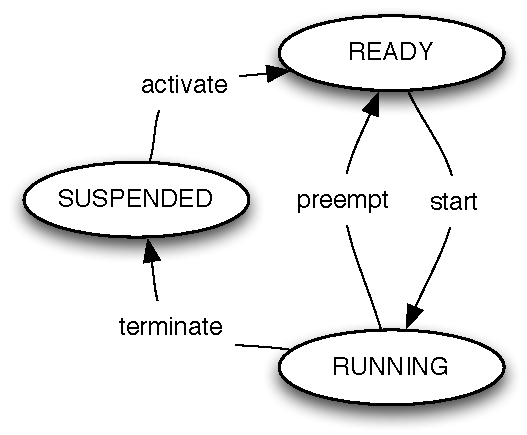
\includegraphics[scale=.6]{pictures/statesBasic.pdf} 
     \caption{States of a \BASIC\ task.}%
     \label{fig:basictaskstates}}%
%   \qquad
   \begin{minipage}{.55\linewidth}%
     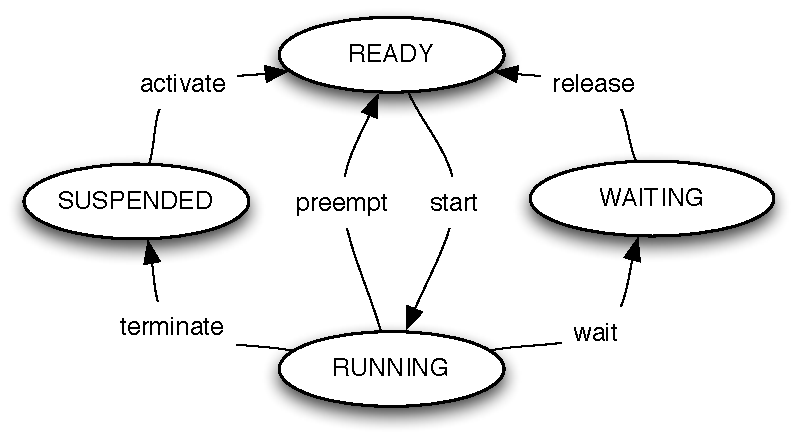
\includegraphics[scale=.6]{pictures/statesExtended.pdf} 
     \caption{States of an \EXTENDED\ task.}%
     \label{fig:extendedtaskstates}%
   \end{minipage}%
\end{figure} 


A task goes from one state to the other according to various conditions as shown in table \ref{tab:statetrans}.

\begin{table}[htbp]
\caption{Transition from state to state of a task.}
\rowcolors{1}{white}{light-gray}
\begin{longtable}[c]{l|l|l|p{7cm}}
\bf transition & \bf former state & \bf new state & \bf description\\
\hline
activate & \SUSPENDED & \READY & the task is set in the \READY\ state on one of the following occurrences: services ActivateTask or ChainTask, activation notification coming from an alarm, a schedule table or a message. \\
start & \READY & \RUNNING & the task is set to the running state and begin to execute because it has the highest priority in the system and has been elected by the scheduler. \\
terminate & \RUNNING & \SUSPENDED & the task is set to the \SUSPENDED\ state when it calls the TerminateTask service.\\
preempt & \RUNNING & \READY & the task is set to the \READY\ state when the scheduler starts a higher priority task.\\
wait & \RUNNING & \WAITING & the task may be set to the \WAITING\ state when it calls the service WaitEvent.\\
release & \WAITING & \READY & the task is set to the \READY\ state when it gets one of the  events it is waiting for. \\
\end{longtable}
\label{tab:statetrans}
\end{table}

\note{A system service may do more than one transition at a time. For instance, if a task is activated by calling \cfunction{ActivateTask} and its priority is higher than the priority of the current running task, the new task will go from \SUSPENDED\ to \RUNNING\ and the intermediate state \READY\ will not be observable.}

\section{The scheduling}
\label{sec:scheduling}

Trampoline schedules the tasks dynamically during the execution of the application. A task is scheduled according to its priority and whether it is preemptable or not. The priority of a task is given at design stage, and indicated in the OIL file using the \PRIORITY\ attribute, see \ref{sec:oiltask}, and may change during execution when the task gets or release a resource. The preemptability of a task may be set too. It is also indicated in the OIL file using the \SCHEDULE\ attribute, see \ref{sec:oiltask}.

A tasks continues to run until it is preempted because a task having a higher priority is put in the \READY\ state,  or it blocks because it is waiting for an event. Only extended tasks may block. If more than one task have the same priority, tasks are run one after the other because a task may not preempt an other task having the same priority. So there is no round robin among tasks of the same priority level.

A non-preemptable task runs until it calls \api{Schedule} and a higher priority task is in the \READY\ state or until it blocks. More informations about priority and preemptability may be found in chapter \ref{chap:resources}.

In the following examples, the horizontal axis is the time.  The state of the task is indicated in a rectangle that spans a period of time. When the task is running the rectangle is grayed. An up arrow \activate\ indicates a task activation and a down arrow \terminate\ a task termination.

\begin{figure}[htbp] %  figure placement: here, top, bottom, or page
   \centering
   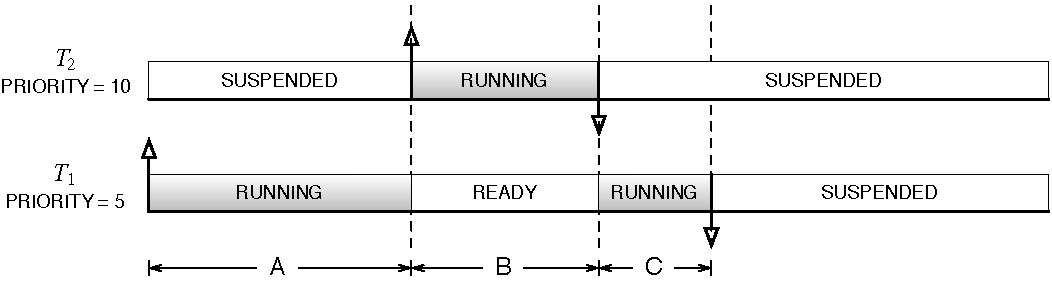
\includegraphics[scale=.7]{pictures/schedulingPreempt.pdf} 
   \caption{{\bfseries Scheduling of preemptable tasks.} During A period, $T_1$ is {\sffamily\scshape running} and $T_2$ is {\sffamily\scshape suspended}. Then $T_2$ is activated. Since $Prio(T_2) > Prio(T_1)$, $T_1$ is preempted and $T_2$ runs (B period). $T_2$ terminates and $T_1$ becomes {\sffamily\scshape running} again (C period) until it terminates.}
   \label{fig:schedulePreempt}
\end{figure} 

\begin{figure}[htbp] %  figure placement: here, top, bottom, or page
   \centering
   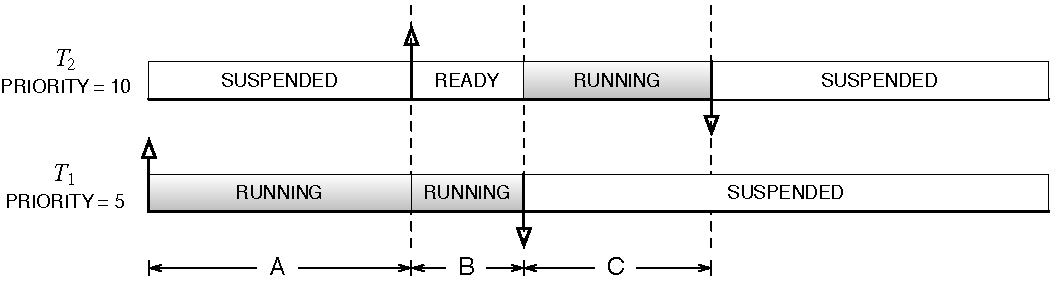
\includegraphics[scale=.7]{pictures/schedulingNonPreempt.pdf} 
   \caption{{\bfseries Scheduling of non-preemptable tasks.} During A period, $T_1$ is {\sffamily\scshape running} and $T_2$ is {\sffamily\scshape suspended}. Then $T_2$ is activated. Even if $Prio(T_2) > Prio(T_1)$, $T_1$ is non-preemptable and continues to run until it terminates (B period). In the meantime, $T_2$ is {\sffamily\scshape ready}. $T_1$ terminates and $T_2$ runs (C period) until it terminates.}
   \label{fig:schedulePreempt}
\end{figure} 

\section{Writing the code of a task}

Trampoline provides a \cmacro{TASK} macro to define a task in a C source file. The macro takes one argument which is the identifier of the task:

%\newpage
\begin{lstlisting}[language=C]
TASK(MyTask)
{
  /* code of the task */
  
  TerminateTask();
}
\end{lstlisting}

The code of the task is plain C.

The task should always end with a call to the \api{TerminateTask} service. See \ref{api:TerminateTask}.


\section{Tasks services}

\begin{service}{DeclareTask}{}

Each task has an identifier of type \ctype{TaskType}. This identifier is declared in the OIL file and is used in system calls to refer to a particular task. Before using such an identifier in your program, you have to declare it:

\begin{lstlisting}[language=C]
DeclareTask(MyTask);
\end{lstlisting}

This makes the \cdata{MyTask} identifier available in the current scope.

\note{ \servicename\ is a C macro. When the task has been define above using the macro \cmacro{TASK}, the identifier of the task is already in the scope and \cmacro{DeclareTask} is not needed.}

\argument{TaskType}{TaskID}{The id of the task to declare}
\end{service}

\begin{service}{ActivateTask}{StatusType}

\note{This service does a rescheduling}

Activates a new instance of a task. If activation counter has reached the maximum activation count or the task cannot be activated for timing protection purpose, the service fails. Otherwise if an instance is already active (\RUNNING\ or \READY), the state does not change and the activation is recorded to be done later. If no instance is active, the state of the task is changed to \READY.

Figures \ref{fig:scheduleT1lp}, \ref{fig:scheduleT1hp} and \ref{fig:scheduleMultiple} show 2 examples of task activation.

\argument{TaskType}{TaskID}{The id of the task to activate}
\resultcode{\OK}{No error, the task has been successfully activated}
\resultcodeext{\OSID}{Invalid TaskID. No task with such an id exists}
\resultcode{\OSLIMIT}{Too many activations of the task}
\end{service}

\begin{figure}[htbp] %  figure placement: here, top, bottom, or page
   \centering
   \begin{minipage}[c]{.6\linewidth}
   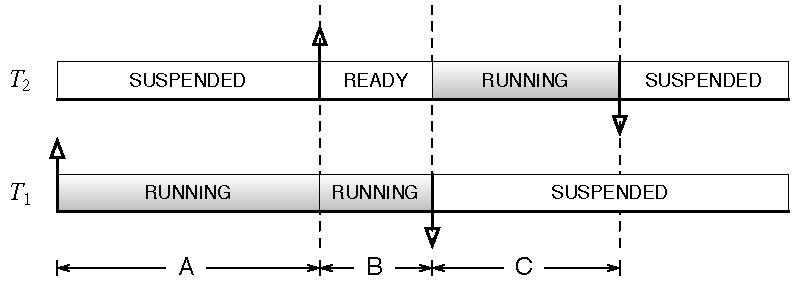
\includegraphics[scale=.7]{pictures/schedulingT1lp.pdf}
   \end{minipage}\hfill
   \begin{minipage}[c]{.3\linewidth}
   \begin{lstlisting}[language=C]
   TASK(T2) {
     ... /* C period */
     TerminateTask();
   }
   
   TASK(T1) {
     ... /* A period */
     ActivateTask(T2);
     ... /* B period */
     TerminateTask();
   }
 \end{lstlisting}
   \end{minipage}
   \caption{{\bfseries Activation of a lower priority task.} $Prio(T_1) \ge Prio(T_2)$. During A period, $T_1$ is {\sffamily\scshape running} and $T_2$ is {\sffamily\scshape suspended}. Then $T_1$ calls {\upshape\ttfamily ActivateTask(T2);}. Since $T_2$ does not have a higher priority, it becomes {\sffamily\scshape ready} (B period).  $T_1$ terminates and $T_2$ runs (C period) until it terminates.}
   \label{fig:scheduleT1lp}
\end{figure} 

\begin{figure}[htbp] %  figure placement: here, top, bottom, or page
   \centering
   \begin{minipage}[c]{.6\linewidth}
   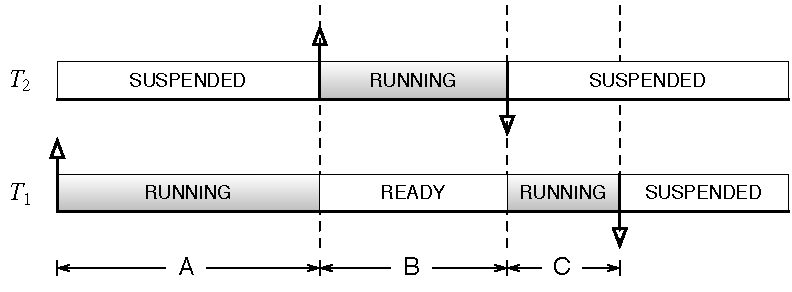
\includegraphics[scale=.7]{pictures/schedulingT1hp.pdf}
   \end{minipage}\hfill
   \begin{minipage}[c]{.3\linewidth}
   \begin{lstlisting}[language=C]
   TASK(T2) {
     ... /* B period */
     TerminateTask();
   }
   
   TASK(T1) {
     ... /* A period */
     ActivateTask(T2);
     ... /* C period */
     TerminateTask();
   }
 \end{lstlisting}
   \end{minipage}
   \caption{{\bfseries Activation of a higher priority task.} $Prio(T_1) < Prio(T_2)$. During A period, $T_1$ is {\sffamily\scshape running} and $T_2$ is {\sffamily\scshape suspended}. Then $T_1$ calls {\upshape\ttfamily ActivateTask(T2);}. Since $T_2$ has a higher priority, it becomes {\sffamily\scshape running} (B period).  $T_2$ terminates and $T_1$ resumes (C period) until it terminates.}
   \label{fig:scheduleT1hp}
\end{figure} 


\begin{figure}[htbp] %  figure placement: here, top, bottom, or page
   \centering
   \begin{minipage}[c]{.6\linewidth}
   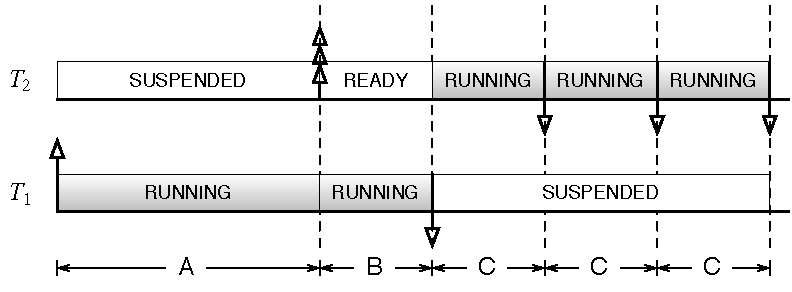
\includegraphics[scale=.7]{pictures/schedulingMultiple.pdf}
   \end{minipage}\hfill
   \begin{minipage}[c]{.3\linewidth}
   \begin{lstlisting}[language=C]
   TASK(T2) {
     ... /* C period */
     TerminateTask();
   }
   
   TASK(T1) {
     ... /* A period */
     ActivateTask(T2);
     ActivateTask(T2);
     ActivateTask(T2);
     ... /* B period */
     TerminateTask();
   }
 \end{lstlisting}
   \end{minipage}
   \caption{{\bfseries Multiple activations of a lower priority task.} $Prio(T_1) \ge Prio(T_2)$. During A period, $T_1$ is {\sffamily\scshape running} and $T_2$ is {\sffamily\scshape suspended}. Then $T_1$ calls {\upshape\ttfamily ActivateTask(T2);} 3 times. Since $T_1$ has a higher priority, $T_2$ does not run immediately and the 3 activations are recorded provided the ACTIVATION attribute in the OIL description of the task is a least 3 (B period). When $T_1$ terminates, the scheduler executes $T_2$ 3 times (C periods).}
   \label{fig:scheduleMultiple}
\end{figure} 



\begin{service}{ChainTask}{StatusType}

\note{This service does a rescheduling}

This service puts task TaskID in \READY\ state, and the calling task in the \SUSPENDED\ state. It acts as the \api{TerminateTask} service for the calling task.
\argument{TaskType}{TaskID}{The id of the task to activate}
\resultcode{\OK}{No error, the task TaskID has been successfully activated and the calling task has been successfully terminated. Note in this case {\ttfamily\servicename} does not return so actually \OK\ is never returned}
\resultcodeext{\OSID}{Invalid TaskID. No task with such an id exists}
\resultcode{\OSLIMIT}{Too many activations of the task}
\resultcodeext{\OSRESOURCE}{The calling task still held a resource}
\resultcodeext{\OSCALLLEVEL}{Called outside of a task}
\end{service}

\begin{figure}[htbp] %  figure placement: here, top, bottom, or page
   \centering
   \begin{minipage}[c]{.6\linewidth}
   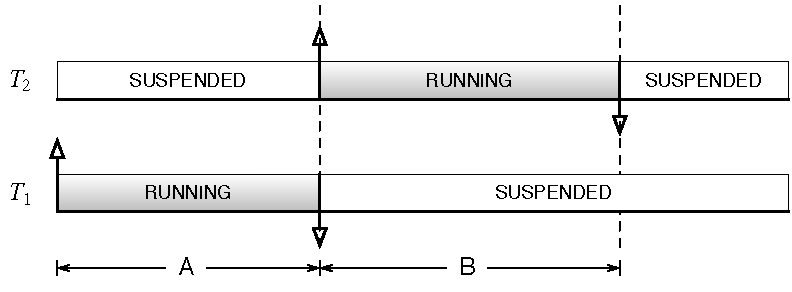
\includegraphics[scale=.7]{pictures/schedulingChain.pdf}
   \end{minipage}\hfill
   \begin{minipage}[c]{.3\linewidth}
   \begin{lstlisting}[language=C]
   TASK(T2) {
     ... /* B period */
     TerminateTask();
   }
   
   TASK(T1) {
     ... /* A period */
     ChainTask(T2);
   }
 \end{lstlisting}
   \end{minipage}
   \caption{{\bfseries Chaining of tasks.} During A period, $T_1$ is {\sffamily\scshape running} and $T_2$ is {\sffamily\scshape suspended}. Then $T_1$ calls {\upshape\ttfamily ChainTask(T2);}. $T_1$ terminates and $T_2$ is activated. Then $T_2$ runs (B periods).}
   \label{fig:scheduleMultiple}
\end{figure} 

\begin{service}{TerminateTask}{StatusType}

\note{This service does a rescheduling}

This service stops the calling task and puts it in \SUSPENDED\ state.
\resultcode{\OK}{No error, the calling task has been successfully terminated. Note in this case {\ttfamily\servicename} does not return so actually \OK\ is never returned}
\resultcodeext{\OSRESOURCE}{The calling task still held a resource}
\resultcodeext{\OSCALLLEVEL}{Called outside of a task}
\end{service}

\begin{service}{Schedule}{StatusType}
\note{This service does a rescheduling. 
Schedule does not deal directly with tasks but since it is a call to the scheduler, it is presented here.}

If called from a preemptable task that does not use an internal resource, Schedule has not effect. If called from a preemptable or a task that uses an internal resource, the priority of the task revert to its base priority and a rescheduling occurs.

Schedule allows to implement cooperative multitasking to insure synchronous rescheduling.
\resultcode{\OK}{No error.}
\resultcodeext{\OSRESOURCE}{The calling task still held a resource}
\resultcodeext{\OSCALLLEVEL}{Called outside of a task}
\end{service}

\begin{service}{GetTaskID}{StatusType}
\cfunction{\servicename} writes in the \var{TaskID} variable passed as reference the identifier of the task currently \RUNNING. If no task is currently \RUNNING\ because \cfunction{\servicename} was called from an ISR of before Trampoline is started, \constant{INVALID_TASK} is got.

\warning{The argument is a pointer. Do not pass an uninitialized pointer. Proper use of this service supposes a \ctype{TaskType} variable is instantiated, then its address is passed to \cfunction{\servicename} as shown in the example below:}

\begin{lstlisting}[language=C]
TaskType runningTaskID;
GetTaskID(&runningTaskID);
\end{lstlisting}

\resultcode{\OK}{No error.}
\resultcodeMP{\OSPROTECTIONMEMORY}{The caller does not have access to the addresses of \var{TaskID} reference} 
\argument{TaskRefType}{TaskID}{Reference to the task}
\end{service}

\begin{service}{GetTaskState}{StatusType}
\cfunction{\servicename} writes in the variable passed as reference in \var{State} the state of the task given in \var{TaskID}.

\warning{The \var{State} argument is a pointer. Do not pass an uninitialized pointer. Proper use of this service supposes a \ctype{TaskState} variable is instantiated, then its address is passed to \cfunction{\servicename} as shown in the example below:}

\begin{lstlisting}[language=C]
TaskStateType T1State;
GetTaskState(T1, &T1State);
\end{lstlisting}

\resultcode{\OK}{No error.}
\resultcodeext{\OSID}{Invalid TaskID. No task with such an id exists}
\resultcodeMP{\OSPROTECTIONMEMORY}{The caller does not have access to the addresses of \var{State} reference} 
\argument{TaskType}{TaskID}{The id of the task.}
\argument{TaskStateRefType}{State}{Reference to the state.}
\end{service}


%\strong{Processes} are both Tasks and ISRs category 2. Trampoline category 2 ISRs are like Basic Tasks except the priority level of the interrupt controller is raised to the priority of the ISR while the later is running.

\section{Inside Task management}
\label{sec:addtaskstate}

\subsection{Static attributes}

A task has the following static attributes:

\begin{description}
\item[The entry point of the task.] A pointer to the code of the task. When the scheduler start a task instance the first time, it uses this pointer to begin the execution.
\item[The internal resource] the task uses if any. An internal resource is automatically taken when a task enters the \RUNNING\ state and automatically released when the task leaves the \RUNNING\ state. See \ref{sec:internalresources} for more informations.
\item[The base priority] of the task as specified in the OIL file. This priority is used to reset the current priority when the task is activated.
\item[The maximum activation count] of the task as specified in the OIL file.
\item[The kind of task,] \BASIC\ or \EXTENDED.
\item[The task id.] Used for internal checking.
\item[The id of the OS Application] the tasks belong to (only available in \autosar\ \SC{3} and \SC{4}).
\item[The timing protection configuration] if any (only available in \autosar\ \SC{2} and \SC{4}).
\end{description}

\subsection{Dynamic attributes}

A task has also the following dynamic attributes:

\begin{description}
\item[The context.] This is the chunk of RAM where the current execution context of a task is stored when the task is in the \READY\ or \WAITING\ state. The execution context is the value of the microprocessor's registers (program counter, stack pointer, other working registers). So the context depends on the target on which Trampoline runs.
\item[The stack(s).] This is the chunk of RAM where registers are pushed for function call. This attributes depends on the target architecture. For instance, the C166 micro-controller uses 2 stacks.
\item[The current activation count.] When a task is activated while not in \SUSPENDED\ state, the activation is recorded and is actually done when the task returns to the \SUSPENDED\ state.  Many activation may be recorded according to the value given to the \oilattr{ACTIVATION} task OIL attribute. When a task is activated, the current activation count is compared to the maximum activation count and if $\ge$, the activation fails.
\item[The list of resources] the task currently owns.
\item[The current priority] of the task. This priority starts equal to the basic priority and may increase when the task get a resource.
\item[The state of the task] as defined in sections \ref{sec:taskstate} and \ref{sec:internaltaskstate}.
\item[The trusted counter.] If $=0$, the task is non-trusted. If $>0$ the task is trusted. See chapter \ref{chap:osapplications} for more informations. This counter is available if Trampoline is compiled with memory protection support.
\item[The activation allowed flag.] If true, the task may be activated. If false, it cannot be activated. This flag is set by the timing protection facility. It is available if Trampoline is compiled with timing protection support. See chapter \ref{chap:timingprotection}.
\end{description}

\subsection{Additional task states}
\label{sec:internaltaskstate}

In addition to states presented in section \ref{sec:taskstate}, 2 extra states are used for internal management: 

\begin{description}
\item[\AUTOSTART] This state is used to indicate what task should be started automatically when \api{StartOS} is called. An \AUTOSTART\ task is in this initial state but no task is in this state once the application code is running. \api{StartOS} iterates through the tasks and activates those that are in the \AUTOSTART\ state.
\item[\READYANDNEW] This state is used to flag a task that is ready but has its context uninitialized. This happens when the task has just been activated. The kernel initializes the context of the task the first time it goes to the \RUNNING\ state.
\end{description}

Figure \ref{fig:states} show a complete task state automaton for both basic and extended tasks with these states added.

\begin{figure}[htbp] %  figure placement: here, top, bottom, or page
   \centering
   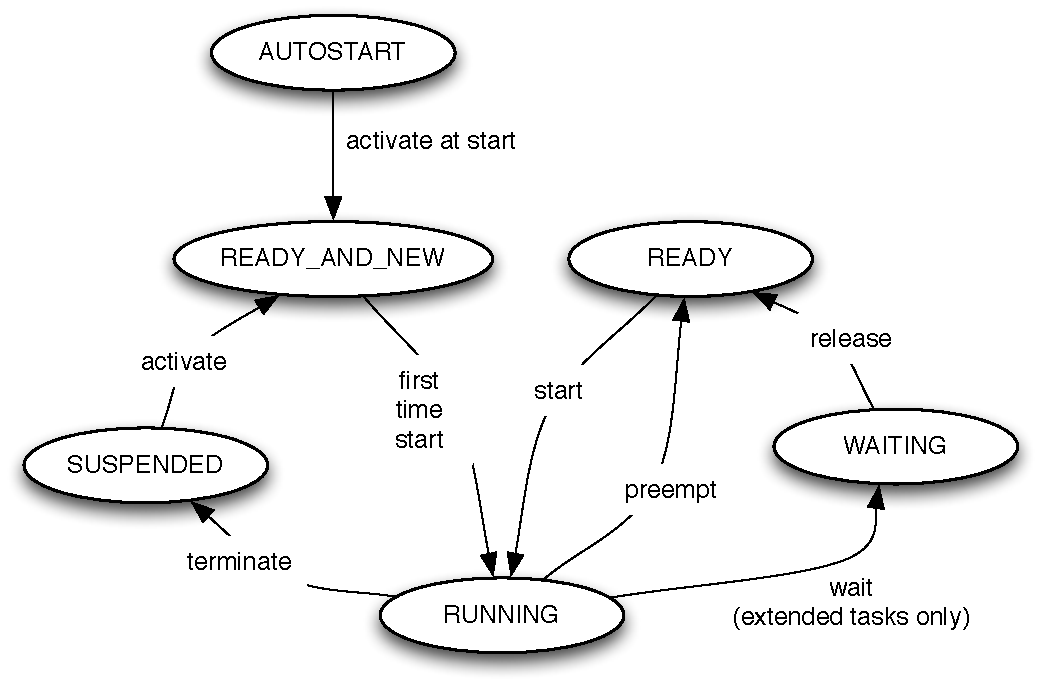
\includegraphics[width=4in]{pictures/states.pdf} 
   \caption{States of a task in Trampoline. \cmacro{AUTOSTART} is the initial state of autostart tasks. \cmacro{SUSPENDED} is the initial state of both non autostart tasks.}
   \label{fig:states}
\end{figure} 


\section{The {\em idle} task}

The {\em idle} task is activated by \api{StartOS}. It is a \BASIC\ task with a priority of 0 (\ie\ the lowest priority in the system, the lowest priority of tasks defined in the application is 1). So when no other task is currently running, the {\em idle} task run.

To be able to use specific platform capabilities (to put the micro-controller in stand by mode for example), this task calls repetitively a hardware specific function called \cfunction{tpl_sleep} (defined in \textit{machines/}). The tasks is then able to quantify the microprocessor occupation.

GOIL doesn't produce anything about this idle task (unlike application(s) task(s)). The idle task descriptor is defined in \file{tpl_os_kernel.c}.